\documentclass{article} 
    %\usepackage[margin=0.8in]{geometry}
    %\usepackage[parfill]{parskip}
    \usepackage[utf8]{inputenc}
    \usepackage{graphicx}
    \usepackage{siunitx}
    \usepackage{amsmath}
    \usepackage{listings}
    \usepackage{color}

%% Define format for matlab source code
\definecolor{dkgreen}{rgb}{0,0.6,0}
\definecolor{gray}{rgb}{0.5,0.5,0.5}
\definecolor{pink}{rgb}{0.63,0.13,0.94}
\lstset{language=Matlab, 
    keywords={break, case, catch, continue,else,elseif,end,for,function,
            global,if,otherwise,persistent,return,switch,try,while},
    basicstyle=\ttfamily,
    keywordstyle=\color{blue},
    commentstyle=\color{dkgreen},
    stringstyle=\color{pink},
    numbers=left,
    numberstyle=\tiny\color{gray},
    stepnumber=1,
    numbersep=10pt,
    backgroundcolor=\color{white},
    tabsize=4,
    showspaces=false,
    showstringspaces=false
}


% Letternumbering
\renewcommand{\thesection}{Part \Alph{section}} 

\title{Artificial Intelligence Methods, exercise 2}
\author{Rendell Cale}
\date{\today}

\begin{document}
\maketitle

\section{}
We can describe the umbrella domain as a hidden Markow model since the  model for the transition from $Rain_{t-1}$ to $Rain_t$ is a Markow process $\mathbf{P}(Rain_t | Rain_{t-1})$. This model, however, is hidden and our window into it is via the "sensor" umbrella. 

\begin{itemize}
    \item Unobserved variable(s): $Rain$
    \item Observable variable(s): $Umbrella$
    \item Dynamic model as matrices:
        \begin{align}
            \mathbf{P}(\mathbf{X}_t | \mathbf{X}_{t-1}) 
                &= \mathbf{P}(\mathbf{R}_t | \mathbf{R}_{t-1}) \\
                &= 
                \begin{bmatrix}
                    0.7 & 0.3 \\
                    0.3 & 0.7
                \end{bmatrix} \\
        \end{align}

        When $Rain_t$ is true, the probability of $Umbrella_t$ being true is $0.9$, and it is $0.2$ when rain is false. This gives the following sensor model. 
        \begin{align}
            \mathbf{P}(\mathbf{E}_t | \mathbf{X}_t) 
                &= \mathbf{P}(\mathbf{U}_t | \mathbf{R}_t ) \\
                &= 
                \begin{bmatrix}
                    0.9 & 0.2 \\
                    0.1 & 0.8 
                \end{bmatrix} \\
        \end{align}
    \item Assumptions: 
        We make three big assumptions in formulating this model. One is that the hidden markov process is a first order Markov process. Given the complexity of weather systems this is probably not going to hold everywhere, but in some locations it may be a reasonable assumption. 

        Another assumption is that the sensor (Umbrella) is only dependent on the current state of the hidden Markov process. This is probably a good assumption since in the example, the directors decission to bring or not bring an umbrella should depend on whether it rained yesterday, only today. 

        The third assumption is that the probabilities don't change with time, so that the system is process is stationary. This can be reasonable over short time spans, but over the course of the year the probabilities should change due to seasons.

\end{itemize}

\section{}
Matlab implementation of Forward algorithm.
\lstinputlisting[language=Matlab]{Forward.m}

Running this function repeatedly as show below on line 14 to 20 gives the following forward result. 

\lstinputlisting[firstline=1,lastline=21,language=Matlab]{tdt4171_ex2.m}

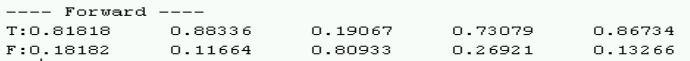
\includegraphics[width=\linewidth]{forward_result.png}
The days read from left to right starting at day 1, so we see that the probability of rain on day 2 was 0.88336 which is what we expected. 


\section{}
Matlab implementation of Backward algorithm.
\lstinputlisting[language=Matlab]{Backward.m}

Running this with the evidence variable equal to $[1\  1]$ gives $\mathbf{P}(\mathbf{R}_1 | \mathbf{e}_{1:2})$.
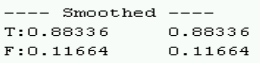
\includegraphics[width=0.4\linewidth]{smoothing_short_result.png}

The probability of rain given the evidence is than 0.88336 according to the Forward-Backward algorithm, which is in accordance with the assignment text. 

Adding evidence for 5 days yeilds the following result.

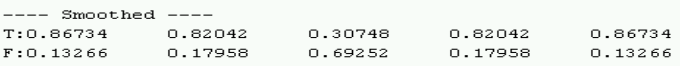
\includegraphics[width=\linewidth]{smoothing_result.png}

From this we can read that the probability of rain on day 1 given the evidence is $0.86734$ (number in top left corner. 


Backward messages are given below.

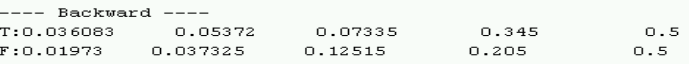
\includegraphics[width=\linewidth]{backward_result.png}



\end{document}

